\chapter{Introduction}\label{Ch:Introduction}

Founded in 1969 as a Silicon valley start-up, Advanced Micro Devices (AMD) is an American company specializing in semiconductor products such as microprocessors, motherboard chipsets and graphic processors. With these products, AMD brings advances in high-performance computing to both IT businesses and consumer markets. In particular, Graphic Processing Units (GPUs) developed and manufactured by AMD empower numerous modifications of gaming consoles including Xbox and PlayStation, thereby contributing to the fast growing gaming industry.\\
\\
According to the statistics published by the Entertainment Software Association, more than 65\% of Americans play video games on at least one type of device \cite{stats}. Furthermore, in 2018 alone, the video game industry produced a revenue of \$43B, an 18\% growth from 2017 \cite{growth}. Therefore, in light of the increasing market share of AMD GPUs---the power source for most gaming devices---it is in AMD's interest to ensure high-quality and error-free gameplay. While games may contain issues of many different sorts, graphics corruption and visual artifacts constitute among the major complaints of users. These artifacts occur as software or hardware errors that alter visual appearance of the game or its individual frames. Figure \ref{fig:bugs} shows some examples of such corruptions as provided by AMD.

\begin{figure}[h]
\centering
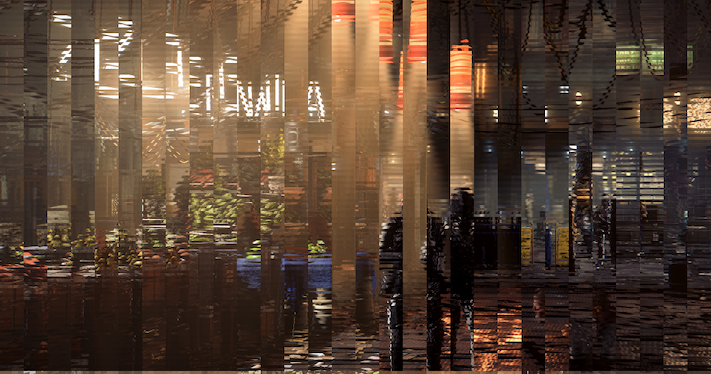
\includegraphics[scale=0.56]{images/bug1new.png}
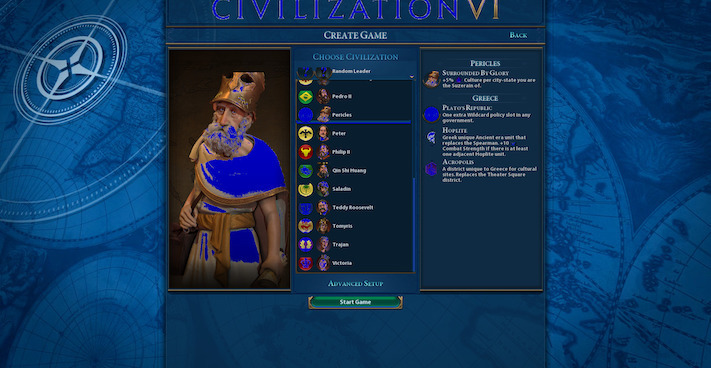
\includegraphics[scale=0.283]{images/bug2new.jpg}\\
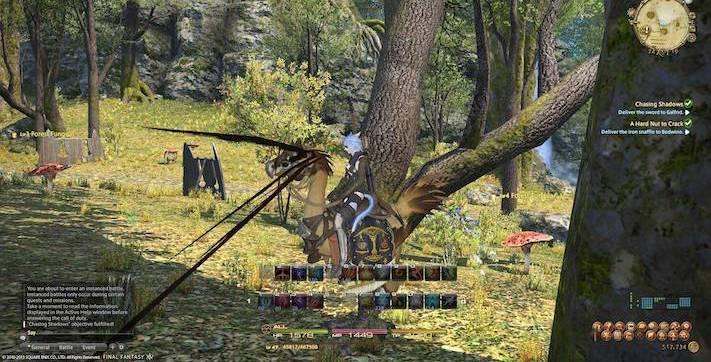
\includegraphics[scale=0.28]{images/bug3new.jpg}
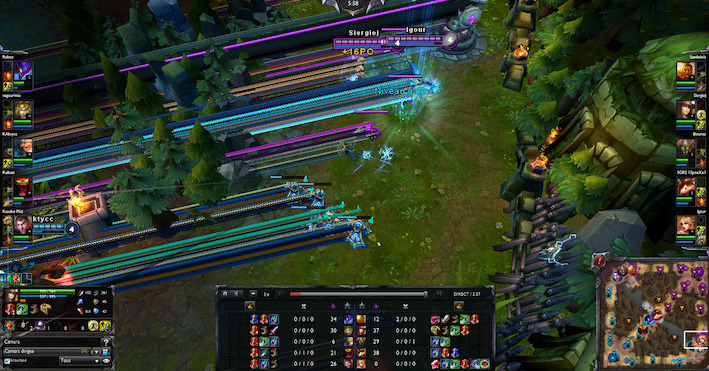
\includegraphics[scale=0.28]{images/bug4new.jpg}\\
\vspace{5pt}
\caption[Examples of video game artifacts]{Examples of video game artifacts (images are courtesy of AMD).}
\label{fig:bugs}
\end{figure}

\noindent
Currently, the task of artifact detection or correction is manual; users report corrupted images to developers or post them in blogs and online forums. Hence, publicly available data is extremely limited, while machine learning algorithms require large datasets for successful training. \\

\noindent In Chapter \ref{Ch:datagen}, we describe our approach at obtaining ``synthetic'' corrupted images using a newly created ``Glitchify'' software that adds certain types of graphics artifacts to normal images. This program was carefully designed to produce 13 different kinds of artifacts that are assumed to occur most frequently. Extraction of relevant features (preprocessing) from the produced data is performed in Chapter \ref{Ch:feature}. Given the characteristics of the 13 artifacts considered in this study, we focused on the discrete Fourier transform, graph Laplacian and pixel-wise anomaly measures. Chapter \ref{Ch:classification} describes designs of models that identify each of the 13 different types of corruptions as well as the assembly of the final ``ensemble'' classifier. Finally, in Chapter \ref{Ch:results} we cover the results that we obtained from our classifiers, yielding a 69\% accuracy on a heldout test set where the games have never been seen by any of the models. We will then wrap up with a discussion of the results and possible sources of bias in Chapter \ref{Ch:discussion}.


\endinput
